Seguindo então para a última das arquiteturas com poucos parâmetros designadas para este trabalho, tem-se os resultados da SqueezeNet dispostos na Tabela \ref{tab:squeezenet}. Mais uma vez a busca em \emph{grid} foi descartada para esta CNN, pelos mesmos motivos considerados para a arquitetura anterior, realizando as mesmas escolhas de hiperparâmetros.

\begin{table}[h!]
\centering
\caption{Detalhamento dos modelos obtidos com a arquitetura SqueezeNet para cada uma das abordagens consideradas neste trabalho.}
\label{tab:squeezenet}
\resizebox{\textwidth}{!}{\begin{tabular}{ccccccc}
\toprule
\textbf{Abordagem} & \textbf{Otimizador} & \textbf{\emph{Patience}}  & \textbf{Função de Ativação} & \textbf{Acurácia} & \textbf{F-Score} & \textbf{EER} \\
\midrule
Abordagem A & RMSprop & 15 & ReLU & $0.9048$ & $0.8948$ & $11.5074$ \\
Abordagem B & RMSprop & 15 & ReLU & $0.8210$ & $0.7709$ & $20.1673$\\
\bottomrule
\end{tabular}}
\end{table}

O histórico de \emph{loss} e acurácia durante o estágio de treinamento destes modelos, disponível na Figura \ref{fig:treinamento-squeezenet}, mostra que, para a abordagem A, a quantidade de épocas atingidas pelo modelo, antes de ocorrer o \emph{early stopping} definido, foi a maior entre todos os modelos aqui representados. Não obstante, é possível notar, também para o modelo da abordagem A, que a sua convergência ocorreu de uma forma mais padronizada, sem muitos altos e baixos na acurácida do conjunto de validação durante o treinamento.
    
\begin{figure}[H]
\centering
\caption{Histórico de \emph{loss} e acurácia durante o treinamento dos modelos obtidos com a arquitetura SqueezeNet.}
\label{fig:treinamento-squeezenet}
\subfloat[\emph{Loss} durante treinamento da rede SqueezeNet para a abordagem A.\label{subfig:squeezenet-a-loss}]{%
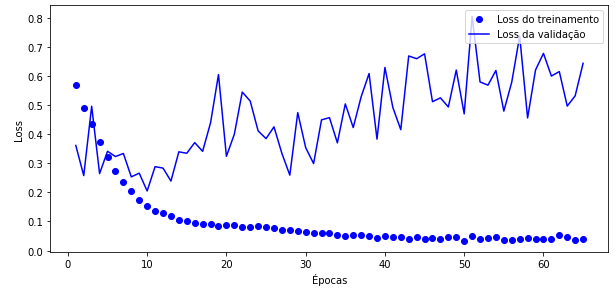
\includegraphics[width=0.47\textwidth]{imgs/squeezenet-a-loss}
}
\hfill
\subfloat[Acurácia durante treinamento da rede SqueezeNet para a abordagem A.\label{subfig:squeezenet-a-acc}]{%
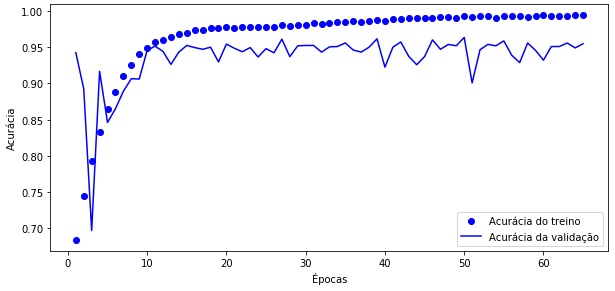
\includegraphics[width=0.47\textwidth]{imgs/squeezenet-a-acc}
}
\hfill
\subfloat[\emph{Loss} durante treinamento da rede SqueezeNet para a abordagem B.\label{subfig:squeezenet-b-loss}]{%
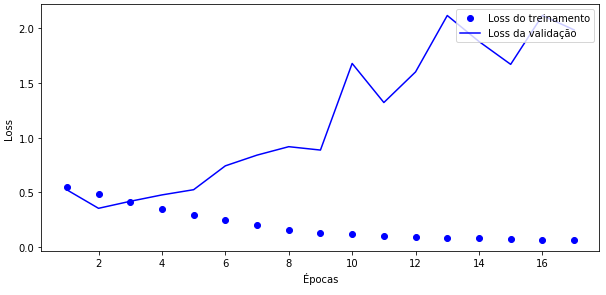
\includegraphics[width=0.47\textwidth]{imgs/squeezenet-b-loss}
}
\hfill
\subfloat[Acurácia durante treinamento da rede SqueezeNet para a abordagem B.\label{subfig:squeezenet-b-acc}]{%
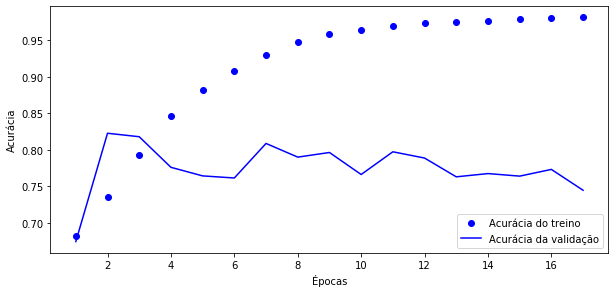
\includegraphics[width=0.47\textwidth]{imgs/squeezenet-b-acc}
}
\end{figure}

Para uma análise mais intensa destes modelos, foram geradas suas matrizes de confusão, demonstradas na Figura \ref{fig:matrizes-squeezenet}. No modelo da abordagem A, é possível utilizar as mesmas reflexões quanto às matrizes obtidas pelas arquiteturas MobileNet e ShuffleNet. Quanto a abordagem B, pode-se verificar a existência de valores parecidos na diagonal secundária da matriz, indicando a presença quase similar de falsos positivos e falsos negativos.
    
\begin{figure}[h]
    \centering
    \caption{Matrizes de confusão dos modelos obtidos com a arquitetura SqueezeNet.}\label{fig:matrizes-squeezenet}
    \subfloat[SqueezeNet com a abordagem A\label{subfig:matriz-squeezenet-a}]{%
    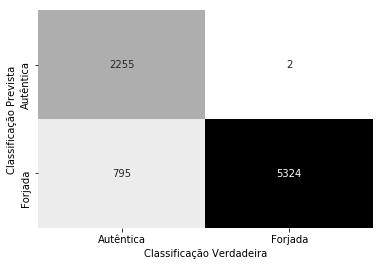
\includegraphics[width=0.47\textwidth]{imgs/matriz-squeezenet-a}
    }
    \hfill
    \subfloat[SqueezeNet com a abordagem B\label{subfig:matriz-squeezenet-b}]{%
    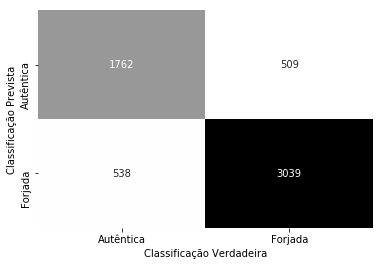
\includegraphics[width=0.47\textwidth]{imgs/matriz-squeezenet-b}
    }
\end{figure}

De maneira geral, apesar do desempenho dos modelos aqui demonstrados terem sido insatisfatórios, é possível perceber que existe ainda a possibilidade de uma busca em \emph{grid} de hiperparâmetros, buscando um modelo com um desempenho similar ou superior aos encontrados até então.